\documentclass{article}

% --- Layout e formattazione generale ---
\usepackage[a4paper, landscape, twocolumn, margin=1.5cm, columnsep=1cm]{geometry}
\usepackage[hidelinks]{hyperref}

% --- Matematica ---
\usepackage{amsthm}
\usepackage{amsmath}
\usepackage{amsfonts}
\usepackage{amssymb}
\usepackage{xcolor}
\numberwithin{equation}{section}
\usepackage{mdframed}
\DeclareMathOperator*{\argmax}{arg\,max}
\DeclareMathOperator*{\argmin}{arg\,min}
\usepackage{cancel}

% --- Teoremi, definizioni e ambienti ---
\renewcommand\qedsymbol{$\blacksquare$}
\newtheorem*{definition}{\color{red}\textbf{Definition}}
\newtheorem*{theorem}{\color{green}\textbf{Theorem}}
\newtheorem*{proposition}{\color{blue}\textbf{Proposition}}
\newmdenv[%
    backgroundcolor=lightgray,
    frametitlebackgroundcolor=gray,
    hidealllines=true,
    frametitlefont=\sffamily\bfseries\color{white},
    frametitle={Example},
]{example}
\newmdenv[%
    backgroundcolor=yellow,
    hidealllines=true
]{recap}

% --- Grafica e disegni ---
\usepackage{graphicx}
\usepackage{wrapfig}
\graphicspath{ {./images/} }


\begin{document}
\pagenumbering{gobble}

\tableofcontents
\clearpage

\pagenumbering{arabic}
\parindent 0pt

\section{Linear Algebra Tools}
This chapter introduces inner product to give geometric meaning to vectors and
vector spaces, enabling calculations of length, distance, and angles.

\begin{definition}[Symmetric Positive Definitive Matrix] 
    A symmetric matrix $A\in \mathbb{R}^{n\times n}$ that satisfies
    \begin{equation}\label{positive_definite_matrix}
        \text{for every nonzero vector }x:x^TAx>0
    \end{equation}    
    is called \textbf{positive definite}. If only $\geq$ holds in
    \ref{positive_definite_matrix}, then $A$ is called \textbf{positive
    semidefinite}.
\end{definition}
These properties helps in identifying positive definite matrices without
having to check the definition explicitly:
\begin{enumerate}
    \item The null space of $A$ contains only the null vector; 
    \item The diagonal elements $a_{ii}$ of $A$ are positive; 
    \item The eigenvalues of $A$ are real and positive.
\end{enumerate}
\subsection{Angles and Orthogonality}
The angle $\omega$ between vectors $x$ and $y$ is computed as:
$$\cos\omega=\frac{\langle x,y\rangle}{\lVert x\rVert_2 \lVert y\rVert_2}$$ 
Here, $\langle x,y\rangle$ denotes the inner product between $x$ and $y$.

This angle indicated the vectors' similarity in orientation. 
\begin{definition}[Orthogonal vectors]
    Two vectors are orthogonal if $\langle x,y \rangle=0$. If additionally
    $\lVert x\rVert=1=\lVert y\rVert$, then $x$ and $y$ are orthonormal.
\end{definition}
\begin{definition}[Orthogonal matrix]
    A square matrix is an orthogonal matrix if and only if \underline{its columns are
    orthonormal} so that 
    $$AA^T=I=A^TA$$
    which implies that 
    $$A^{-1}=A^T$$
\end{definition}
The length of a vector $x$ is not changed when transforming it using an
orthogonal matrix $A$.
$$\lVert Ax\rVert_2^2=\lVert x\rVert_2^2$$
Moreover, the angle between any two vectors $x,y$ is also unchanged when
transforming both of them using an orthogonal matrix $A$.
\begin{definition}[Orthonormal Basis]
    In an $n$-dimensional vector space $V$ with a basis set
    $\{b_1,\ldots,b_n\}$, if all the basis vectors are orthogonal to each
    other, the basis is called as an \textbf{orthogonal basis}.
    Additionally, if the length of each basis vector is 1, the basis is
    referred to as an \textbf{orthonormal basis}.
\end{definition}
We can also have vector spaces that are orthogonal to each other. Given a
vector space $V$ of dimension $D$, let's  consider a subspace $U$ of dimension
$M$ such that $U\subseteq V$. Then its \textbf{orthogonal complement}
$U^{\perp}$ is a $D-M$ dimensional subspace $V$ and contains all vectors in
$V$ that are orthogonal to every vector in $U$.
\begin{center}
    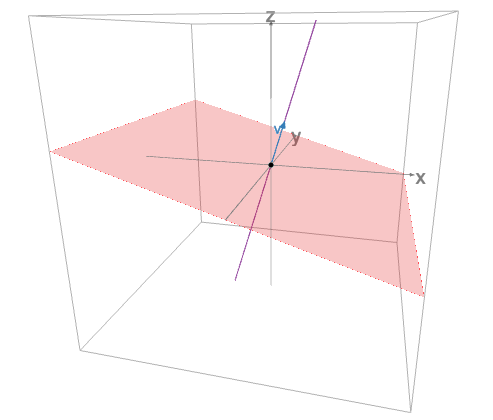
\includegraphics[width=0.6\linewidth]{images/orthogonal_complement}
\end{center}
\subsubsection{Orthogonal Projections}
Projections are key linear transformations in machine learning and are
particularly useful for handling high-dimensional data. Often, only a few
dimensions in such data are essential for capturing the most relevant
information. By projecting the original high-dimensional data onto a lower
dimensional feature space, we can work more efficiently to learn about the
dataset and extract significant patterns.
\begin{definition}[Projection]
    Let $V$ be a vector space and $U\subseteq V$ a subspace of $V$. A linear
    mapping $\pi:V\to U$ is called \textbf{projection} if it satisfies
    $\pi^2=\pi\circ\pi=\pi$.
\end{definition}
Given that linear mappings can be represented by transformation matrices, the
above definition extends naturally to \textit{projection matrices} $P_{\pi}$.
These matrices exhibit the property that $P_{\pi}^2=P_{\pi}$.

The projection $\pi_U(x)$ of a vector $x\in \mathbb{R}^n$ onto a subspace $U$
is the closest point necessarily in $U$ to $x$.
\section{Matrix Decompositions}
\subsection{Eigenvalues and Eigenvectors}
Eigenanalysis helps us understand linear transformations represented by a
matrix $A$. Eigenvectors $x$ are special vectors that only get scaled, not
rotated, when multiplied by $A$. The scaling factor is the eigenvalue
$\lambda$, which indicated how much $x$ is stretched or shrunk. $\lambda$ can
also be zero.
\begin{definition}[Eigenvalue and Eigenvector]
    Let $A\in \mathbb{R}^{n\times n}$ be a square matrix. Then $\lambda\in
    \mathbb{R}$ is an \textbf{eigenvalue} of $A$ and nonzero vector $x$ is the
    corresponding \textbf{eigenvector} of $A$ if 
    \begin{equation}\label{eq:eigenvalue_equation}
        Ax=\lambda x
    \end{equation}
    We call \ref{eq:eigenvalue_equation} the \textbf{eigenvalue equation}.
\end{definition}
The following statements are equivalent:
\begin{itemize}
    \item $\lambda$ is an eigenvalue of $A\in \mathbb{R}^{n\times n}$.
    \item A nonzero vector $x$ exists such that $Ax=\lambda x$ or,
        equivalently, $(A-\lambda I_n)x=0$ for $x\neq 0$.
    \item Then $A-\lambda I$ is a \textbf{singular
        matrix} and its determinant is \textbf{zero}.
\end{itemize}
Each eigenvector $x$ has one unique eigenvalue $\lambda$, but each $\lambda$
can have multiple eigenvectors.
\begin{definition}[Eigenspace and Eigenspectrum]
    For $A\in \mathbb{R}^{n\times n}$, the set of all eigenvectors of $A$
    associated with an eigenvalue $\lambda$ spans a subspace of
    $\mathbb{R}^n$, which is called the \textbf{eigenspace} of $A$ with
    respect to $\lambda$ and is denoted by $E_{\lambda}$. The set of all
    eigenvalues of $A$ is called the \textbf{eigenspectrum} of $A$.
\end{definition}
\begin{definition}
    Let $\lambda_i$ be an eigenvalue of a square matrix $A$. Then the
    \textbf{geometric multiplicity} of $\lambda_i$ is the number of linearly
    independent eigenvectors associated with $\lambda_{i}$. In other words, it
    is the dimensionality of the eigenspace spanned by the eigenvectors
    associated with $\lambda_i$.
\end{definition}
\begin{theorem}
    The eigenvectors $x_1,\ldots,x_n$ of a matrix $A\in \mathbb{R}^{n\times
    n}$ with $n$ distinct eigenvalues $\lambda_1,\ldots,\lambda_n$ are
    linearly independent.
\end{theorem}
This theorem states that eigenvectors of a matrix with $n$ distinct eigenvalues
form a basis of $\mathbb{R}^n$.
\end{document}
